In this section we pursue with the analysis of data scrapped on several cryptocurrency subreddits. More precisely, we use social media analytics on the network that we built in the previous section. Firstly, we investigate if our network follows a power law distribution as it should. Secondly, we discuss the results of the PageRank algorithm on the network. Thirdly, we run Louvain community detection algorithm and compare the results with the existing subreddits. And finally we analyse the price development of the Bitcoin and try to find a correlation with our data.

\subsection{Power Law Distribution}

The power law distribution in a network can be understood as ``a few users are very popular and a lot of users are mildly or not popular at all''. Intuitively, this relation holds in our network composed of vertices as users and edges representing the comment relation. Indeed, when browsing Reddit in general, we may notice that a few comments (users) are very popular (have a very high score) as others are not. This intuition reveals itself true when plotting the node degree distribution (see fig. \ref{fig:degdist}). This is encouraging in relation to our network model and further analysis because natural networks tend to follow that law. It therefore means that our network is properly formed that the analysis that follows is most likely consistent natural laws.
\begin{figure}[H]
    \centering
    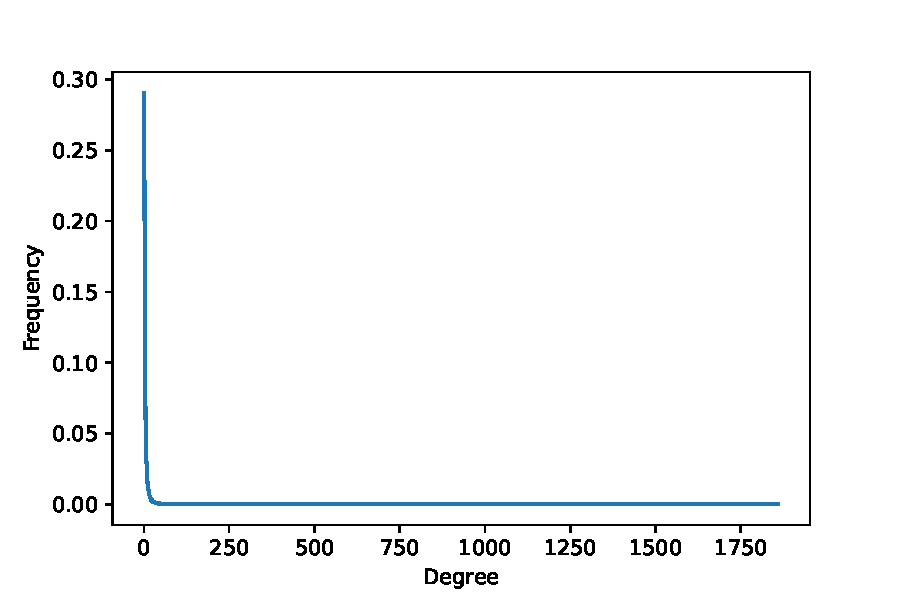
\includegraphics[width=0.3\textwidth]{figures/deg_dist.pdf}
    \caption{The network follows a power law distribution: a lot of users have few comments on their posts and a few users have a lot of comments on their posts.}
    \label{fig:degdist}
\end{figure}



\subsection{Page Rank}

Regarding PageRank (PR), it can be interpreted as the amount of random walks in the network that end up on a particular vertex. For our network, it means that the higher the rank of one user is, the higher the probability is of commenting one post of that particular user. We decide here to investigate the steadiness of PR over 15 days. We might observe unsteadiness on figure \ref{fig:rankdays} but this is not entirely true with respect to the PageRank. First, this is true that the graph evolves quite rapidly over the days. The same users will not necessarily be active twice on the same comment over multiple days. This observation has been done by computing the set of users over the days and devising the similarity for each successive day. Let $U_i$ be the set of users for day $i$, then $s\left(i,j\right)$ is the similarity between day $i$ and $j$ such that $$s\left(i,j\right)=\frac{U_i\cap U_{j}}{U_i\cup U_{j}}.$$ We get the graph at figure \ref{fig:simdays}. However, the PR itself seems to be pretty consistent over the days when we compute the sum of the squared error between the intersected PR values as shown in graph \ref{fig:errordays} where the error only spikes to a value of $0.005$. We can conclude from these two observations that, although there are few overlapping users over the days, the ones that overlap tend to be very popular for a long period. This also means that in the cryptocurrency subreddits, posts tend to have a lasting interest for the users. This conclusion is consistent with the paper \cite{glenskiCharacterizingSpeedScale2019} where they state that cryptocurrencies discussion are likely to trigger a longer lasting discussion.
\begin{figure}[H]
    \centering
    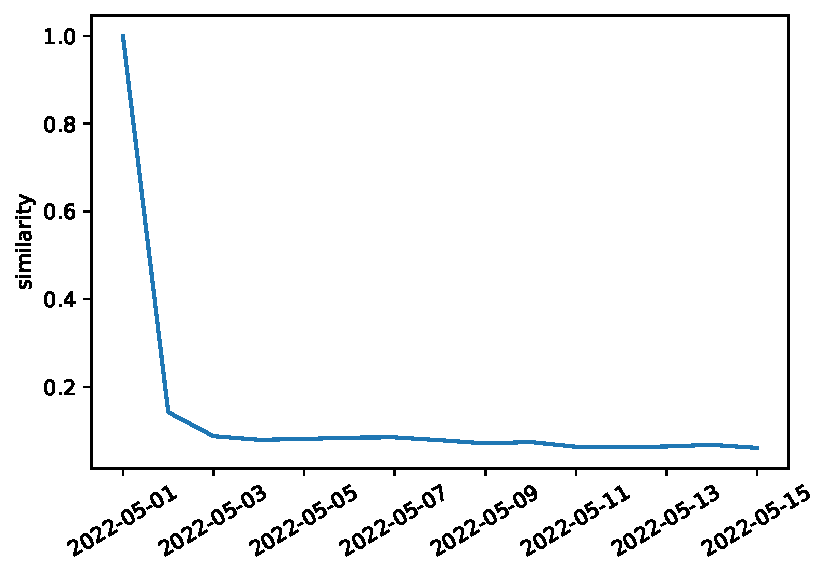
\includegraphics[width=0.3\textwidth]{figures/sim_days.pdf}
    \caption{Similarity between user sets over the 1st to the 15th May.}
    \label{fig:simdays}
\end{figure}
\begin{figure}[H]
    \centering
    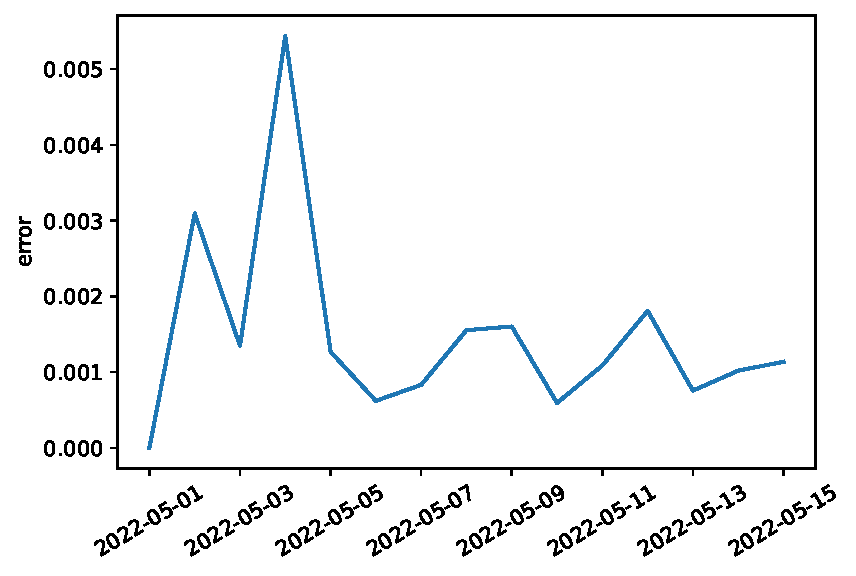
\includegraphics[width=0.3\textwidth]{figures/error_days.pdf}
    \caption{Sum of the squared error of PageRank values over intersected user sets between the 1st and the 15th May.}
    \label{fig:errordays}
\end{figure}

\begin{figure}[H]
    \centering
    \includegraphics[width=0.5\textwidth]{figures/rank_days.pdf}
    \caption{Networks between the 1st to the 15th May. The size of the nodes is relative to the PageRank values.}
    \label{fig:rankdays}
\end{figure}

\subsection{Louvain}
Louvain method is a technique that find communities from large networks. In our case, we were interested to see the communities of our network and observe the links with the different subreddits. To do this, we first create a list of communities corresponding to each subreddit. Each person is assigned to a single community, the one where he/she has interacted the most. Then, we create a second list of communities by applying the Louvain method on the graph based on the \textit{Deep Link No Merge} data model.
After this, we get a list of 260 communities. Knowing that there are 10 subreddits, one subreddit can therefore have several inner communities. 

It can also be interesting to know if some communities are formed by people from different subreddits. For this, we loop over the Louvain communities and compute the percentage of people coming from each subreddit. As a result matrix where rows are Louvain communities and columns are the percentage of people from each subreddit. To have a better understanding of the result, we can plot a histogram of the number of different subreddits that people in a Louvain community belong to (see figure \ref{fig:louvainrepartition}).

\begin{figure}[H]
    \centering
    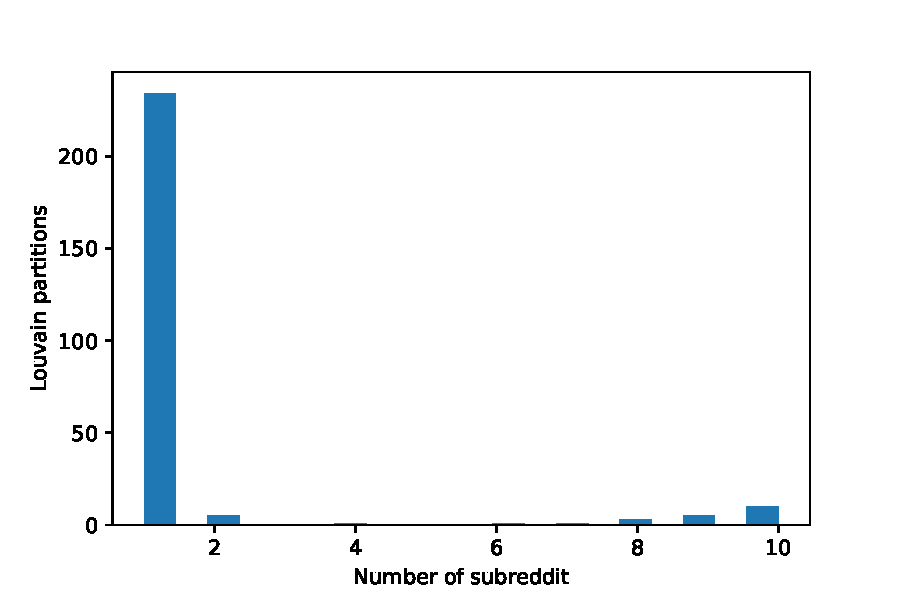
\includegraphics[width=0.3\textwidth]{figures/inner_communities_repartition.pdf}
    \caption{Repartition of Louvain communities in the subreddits.}
    \label{fig:louvainrepartition}
\end{figure}

With this histogram, we can observe that for the majority, the Louvain communities are formed by people from the same subreddit. However, there is also some Louvain communities that are not restricted to one subreddit but are even made up of people from all 10 subreddits.

\subsection{Correlation to price development}

We wanted to capture the activity of our data. To do so, we group our data by some time window; we chose 1 hour. We create a graph $G_0$ from the first time window. Then we create a second graph $G_1$ from the first union second time window. We continue until we have an inclusion sequence such that 
$$ G_0 \subset G_1 \subset  ... \subset G_{n-1},$$

where $n$ is the number of time windows, and $G_i$ a graph based on the \textit{Deep Link No Merge} data model.
Then, we use the degree centrality to compare each graph with its subsequent graph. This results into a table where we have for each user (node) the development of its activity (degree). With this huge dataset, it is now possible to track users and also identify the most active users. However, since this requires lots of computation power and much more work to get something meaningful from this, we opted for the option to sum each time frame (e.g. 1 hour in our case). 

\begin{figure}[H]
    \centering
    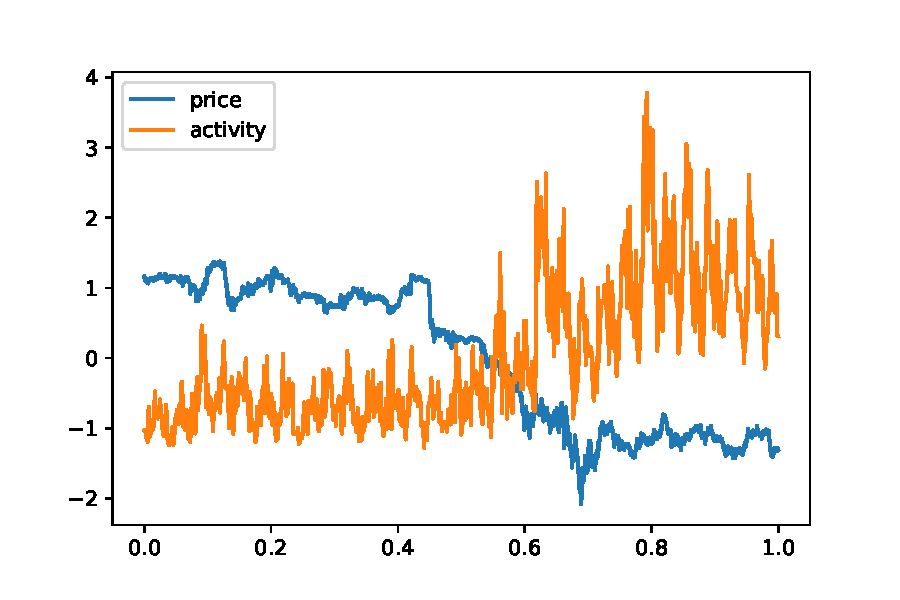
\includegraphics[width=0.5\textwidth]{figures/activity_x_price.pdf}
    \caption{The Reddit activity and the BTC price, normalized, from 01.04 to 22.05.2022.}
\end{figure}


We're now at that stage where one could run some correlation method on our summed activity dataset against the price data. However, this will not yield good results as both datasets are very volatile. Therefore we needed to smoothen our data somehow. We opted for the moving window average method. We took both datasets and computed moving window averages with step 2, 3, 4, ..., 30. These steps represent the number of columns that will be averaged. 

Then, we compared each activity moving window average for each price moving window average using two of pandas built-in correlation methods, namely Pearson, Spearman and we also tried the The Hilbert–Schmidt independence criterion (HSIC). The first two methods deliver strong correlation coefficients (around -0.85), while the HISC does not. Also, we notcied that the correlation differs depending on how much days (from when to when) we try to correlate. We've found that more than 10 days usually yields better results. Please refer to the interactive notebook for details.

\begin{figure}[H]
    \centering
    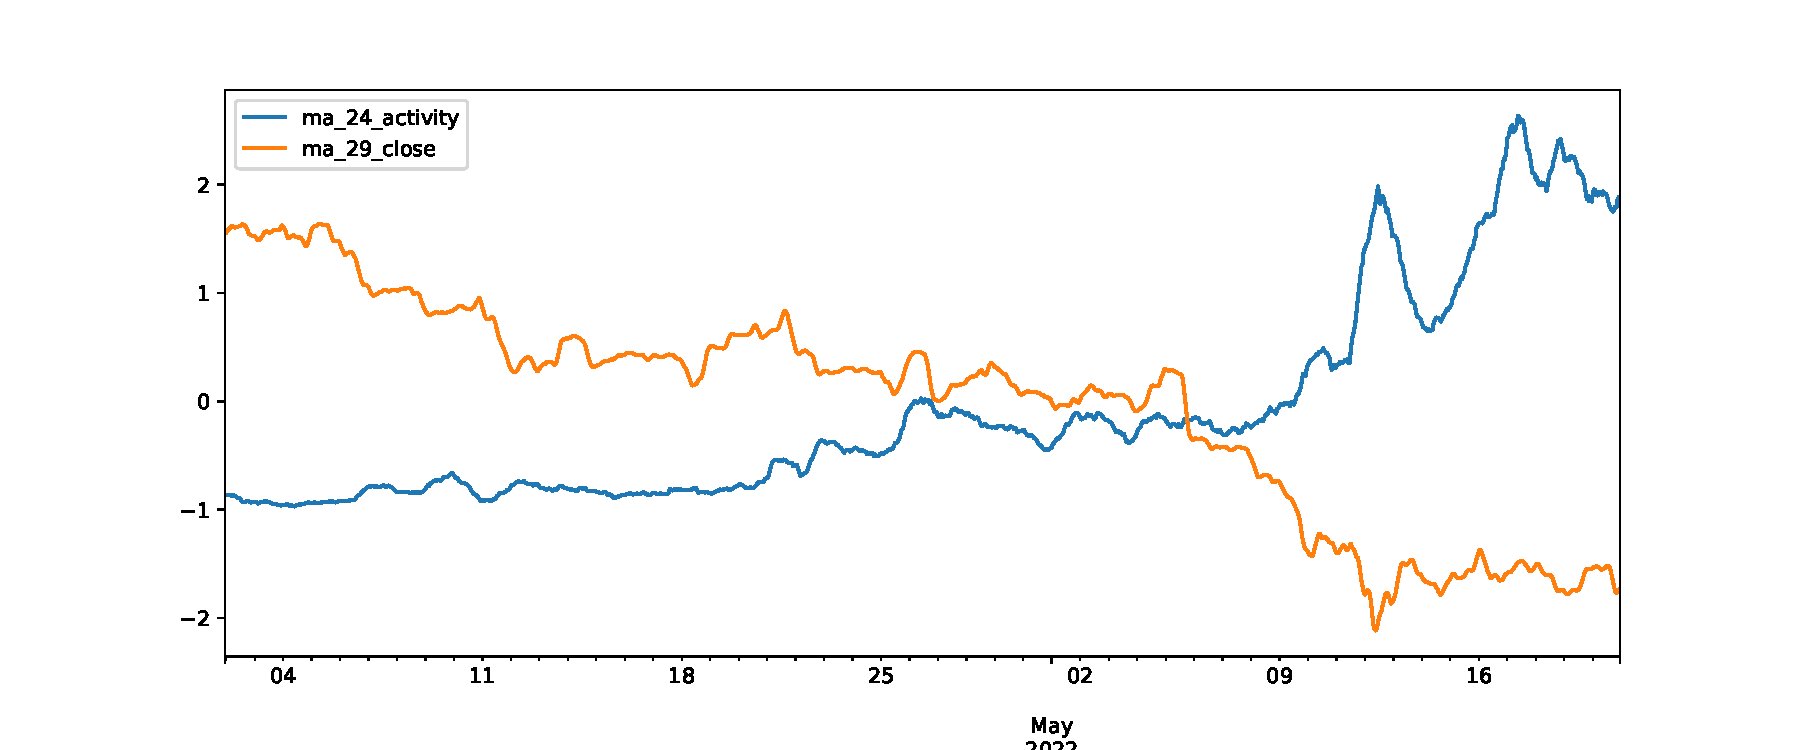
\includegraphics[width=0.5\textwidth]{figures/corr_pearson_0.pdf}
    \caption{Moving averages of the BTC price and the Reddit activity. Pearson Correlation yields a value of -0.889.}
\end{figure}

%% ADDED BY FX AFTER READING CITED PAPER

However, it is important to remember that a correlation between two sets of data does not necessarily indicate a causal link. Here we rely on the results given by paper \citetitle{wooleyExtractingCryptocurrencyPrice2019} and assume that there is a causal link. \citeauthor{wooleyExtractingCryptocurrencyPrice2019} have indeed been able to prove a causal link between price movements and Reddit activity notably with bivariate Granger causality tests. Furthermore, the results shown above are consistent with \citetitle{iderCryptocurrencyReturnPrediction2022} where the authors are able to predict a future price changes with an accuracy significantly better than random guesses \cite{iderCryptocurrencyReturnPrediction2022}.



